% JSSA Report Template for English ver.200908
% By Daichi Ando
% based on ICMC2005

\documentclass{article}
\renewcommand{\baselinestretch}{0.9}
\usepackage{jssa_e,amsmath}
\usepackage{mediabb}
\usepackage{graphicx}

% \usepackage[style=authoryear,firstinits=true]{biblatex}
\usepackage[]{biblatex}
\addbibresource{SpatDIF.bib}

% Title.
% ------
\title{Implementing the SpatDIF Library}

% Paper Category
\category{Short Paper}

% Single address
% To use with only one author or several with the same address
% ---------------
%\oneauthor
%  {Author Name} {Faculty of Fine
%  Arts, Tokyo University of the Arts}

% Two addresses
% --------------
\twoauthors
  {Chikashi Miyama} {Department \\ School}
  {Jan C. Schacher} {Zurich University of the Arts \\ Institute for Computer Music and Sound Technology\\Baslerstrasse 30, Zurich, Switzerland\\jan.schacher@zhdk.ch}

% Three addresses
% --------------
%\threeauthors
%  {First author} {School \\ Department}
%  {Second author} {Company \\ Address}
%  {Third author} {Company \\ Address}

\begin{document}
%
%%% -- Page Number Designation
% Ignore when submitting

\makeatletter 
\def\ps@myheadings{% 
\let\ps@jpl@in\ps@plain% 
\def\@evenhead{\reset@font\hfil\leftmark\hfil}% 
\def\@oddhead{\reset@font\hfil\rightmark\hfil}% 
\let\@mkboth\@gobbletwo% 
\let\sectionmark\@gobble% 
\let\subsectionmark\@gobble% 
% 
\def\@oddfoot{\reset@font\hfil-- \thepage --\hfil}% 
\let\@evenfoot\@oddfoot 
} 
\makeatother 
%%% 
%%% Designation of starting page number
% Ignore when submitting
\setcounter{page}{17} 
\pagestyle{myheadings} 
%%%
% Designation of header
% Ignore when submitting
\markright{\footnotesize \sl Journal of the Japanese Society for Sonic Arts, Vol.1 No.1 pp.17--21} 
%%% 
%%% \maketitleの直後の行に \thispagestyle{myheadings} を挿入する。 
\maketitle
\thispagestyle{myheadings}

\begin{abstract}

Here we have an abstract

\end{abstract}

\section{Introduction}


\section{history of the project} %assigned to Jasch
SpatDIF was coined in \cite{peters_caa07} when Peters stated the necessity for a format to describe spatial sound scenes in a structured way, since at that time the available spatial rendering systems all used self-contained syntax and data-formats. 
Through a panel discussion \cite{2008ICMCpanel, Peters:2008spatdif} and other meetings and workshops, the concept of SpatDIF has since been extended, refined, and consolidated. 

After a long and thoughtful process, the SpatDIF specification was informally presented to the spatial sound community at the ICMC 2011 in Huddersfield in August 2011, at a workshop at the TU-Berlin in September 2011 and in its current form in a Computer Music Journal article in 2013 \cite{}
The responses in these meetings suggested the urgent need for a lightweight and easy to implement spatial sound scene standard, which could contrast the complex MPEG specification \cite{scheirer1999audiobifs}.  
In addition, many features necessary to make this lightweight standard functional were put forward, for example the capability of dealing with temporal interpolation of scene descriptors. 

\section{conceptual explanation / structure} %assigned to Jasch/Trond/Nils

what is SpatDIF?

score-example in XML / JSON

format of SpatDIF `bundle'

\section{current activities} %assigned to Jasch/Trond/Chikashi

\section{library details/structure} %assigned to Chikashi

definition/features/tasks of the lib

interfaces in/out $\rightarrow$ (native C/C++ / OSC)

class structure


fileparsing XML/JSON

OSC 1.0

how to query in 3 lines (C++ code snippet)

\section{reference renderer }% Jasch

The SpatDIF library is complemented with an Application that serves as a reference implementation and test-platform or a real-world usage of spatDIF files. It can validate spatdif-files in XML and JSON formats and be used to check OSC-formatted network streams of SpatDIF statements.
The

app scope / what does it do

app interfaces to lib $\rightarrow$ task distribution between app and lib

i.e. scheduler

or sockets / file-IO

% presentatio structure:

% motivation
% syntax/coneptual development
% the lib / actual implementation
% demo

\printbibliography

% \bibliographystyle{plain}
% \begin{thebibliography}{citations}
% \bibitem{Author1:08} Henoheno Moheji {\it The Book of Computer Music},
% 	Mingmei Publishing, 2008.
% \bibitem{Author2:09} Harahoro Hirehare ``The Abstract of The Book of
% 	Computer Music'', {\it Comtemporary Computer Music Society},
% 	Vol.2 No.4, pp22-26, 2009.
% \end{thebibliography}

\section{Author's Profile}


\subsection*{Author's Name}

\end{document}

% TODO spatfdif-lib paper
% 
% - history  of the project Jasch
% - conceptual explanation / structure Jasch/Trond/Nils
% - current activities Jasch/Trond/Chikashi
% - library details/structure Chikashi
% - reference renderer (rough sketch....) Jasch
% 
% JSSA presentation dec 7. 
% paper deadline nov 7.
% 
% paper finished nov 4.
% 
% milestones:
% 7. october first sketches structure, (blocks of text)
% 21. october finished textblocks
% 4. november finished with all the refs. corrected submittable
% 




Use basic \LaTeX commands.

Headings are as follows:

\subsection{subsection}

This is \verb|\subsection{}|.

\subsubsection{subsubsection}

This is \verb|\subsubsection{}|.

\section{Include Figures}

The way to insert figures is as follows:

\begin{figure}[h]
\centerline{
	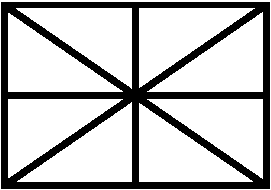
\includegraphics[mediaboxonly,width=\columnwidth]{figure.pdf}}
\caption{English Caption.}
\label{fig:figure}
\end{figure}

Giving [h] option, insert a figure at the specified position.

\section{Foot Note}

The way to insert footnote is as follows\footnote{This is foot note}.

\section{Citiation}

This is citiation\cite{Author1:08}.

Also multiple citiation is as follows\cite{Author1:08,Author2:09}.

\section{For Count Number of Characters}


	
\printbibliography

% \bibliographystyle{plain}
% \begin{thebibliography}{citations}
% \bibitem{Author1:08} Henoheno Moheji {\it The Book of Computer Music},
% 	Mingmei Publishing, 2008.
% \bibitem{Author2:09} Harahoro Hirehare ``The Abstract of The Book of
% 	Computer Music'', {\it Comtemporary Computer Music Society},
% 	Vol.2 No.4, pp22-26, 2009.
% \end{thebibliography}

\section{Author's Profile}


\subsection*{Author's Name}

Author's Profile. Author's Profile. Author's Profile. Author's
Profile. Author's Profile. Author's Profile. Author's Profile. Author's
Profile. Author's Profile. Author's Profile. Author's Profile. Author's
Profile. Author's Profile. Author's Profile. Author's Profile. Author's
Profile. Author's Profile. Author's Profile. Author's Profile. Author's
Profile. Author's Profile. Author's Profile. Author's Profile. Author's
Profile. Author's Profile. Author's Profile. Author's Profile. Author's
Profile. Author's Profile. Author's Profile. Author's Profile. Author's
Profile. 



\end{document}

